\chapter{PEOPLE: Predetermined Order, Pruned Label}\label{chapter:peopel}

Wie im \autoref{chapter:kontraktion} diskutiert wurde, ist Kontraktion von Graphen mit hohem durchschnittlichem Knotengrad aufwendig.
Vielleicht ist die Kontraktion von ihnen sogar so aufwendig, dass sie sich nicht in sinnvoller Zeit kontrahieren lassen.
Trotzdem wäre es praktisch, wenn sich die Anfrage-Zeiten von Contraction-Hierarchies und Hierarchical Hub Labeling auch auf sie übertragen ließen.
Hierfür charakterisieren wir den Contracted- und Hub-Graphen neu und stellen anschließend PEOPLE (\textbf{P}redetermined \textbf{O}rder, \textbf{P}runed \textbf{L}ab\textbf{e}l) vor, eine Methode wie Hub- und Contracted-Graphen mit einer vorgegebenen vertex-to-level-Funktion ohne Knoten-Kontraktion erstellt werden können.

\section{Contracted-Graph}

Um die nachfolgende Definition vorzubereiten, betrachten wir ein Beispiel.
Sei $G = (V, E)$ mit $V \supset \{ u, v, w \}$ und $E = \{ (u, v, {spd}((u, v))), (v, w, {spd}((v, w))) \}$, ein Produkt einer Kontraktion, also zu Beginn mehr Kanten und nicht-isolierte Knoten enthält
Es soll nun $v$ kontrahiert werden.
Hierfür wird eine Kante $(u, w, {spd}((u, w)))$ eingefügt und die Kanten $(u, v), (v, w)$ entfernt.
Daraus können zwei Folgerungen gezogen werden:

\begin{enumerate}
  \item
        Es gibt einen kürzesten Pfad von $u$ nach $w$ in $G$ für den gilt, dass alle Knoten zwischen $u$ und $w$ bereits kontrahiert wurden.
        Diese haben daher auch ein niedrigeres Level als $u$ und $w$.

  \item
        $(u, w) \in E_u$ gilt genau dann, wenn $w$ das größte Level auf allen Pfaden von $u$ nach $w$ hat.
        $(w, u) \in E_d$ gilt, wenn $u$ das größte Level hat.
\end{enumerate}

Basierend auf dieser Überlegung, definieren wir den Upward-Graph neu.

\begin{definition}[Upward-Graph]\label{people:def:upward_graph}
  Sei $G = (V, E)$ und ${vtl}$ eine vertex-to-level-Funktion dazu.
  Dann ist $G_u = (V, E_u)$ ein \emph{Upward-Graph} zu $G$, wenn für jeden Knoten $t \in V$ gilt:

  \begin{itemize}
    \item
          $E_u$ enthält nur Kanten $(t, h, d)$ mit $h \in V$ und $d \in \mathbb{R}^+$, für die es einen $t$-$h$-Pfad der Länge $d \geq {spd}_G (t, h)$ gibt, so dass auf ihm $h$ das größte und $t$ das zweitgrößte Level hat.

    \item
          $E_u$ enthält alle Kanten $(t, h, {spd}_G (t, h))$ mit $h \in V$, für die gilt, dass auf \emph{allen} $t$-$h$-Pfaden $h$ das größte und $t$ zweitgrößte Level hat.
  \end{itemize}
\end{definition}

Betrachten wir dies wieder am Beispielgraph.
Sei ${vtl}$ durch die Abbildung in \autoref{ch::fig::vtl_abbildung} definiert.
Durch Anwendung der neuen Definition des Upward-Graph ergibt sich der in \autoref{ch::fig::upward_graph} gezeigte Graph.

\begin{table}[ht]
  \centering
  \begin{tabular}{lllllllllllll}
    Vertex & a & b & c & d & e & f & g & h & i & j  & k & \\
    Level  & 8 & 7 & 3 & 6 & 2 & 5 & 1 & 4 & 0 & 10 & 9 &
  \end{tabular}
  \caption{${vtl}$ Beispielfunktion}
  \label{ch::fig::vtl_abbildung}
\end{table}

\begin{figure}[ht]
  \centering
  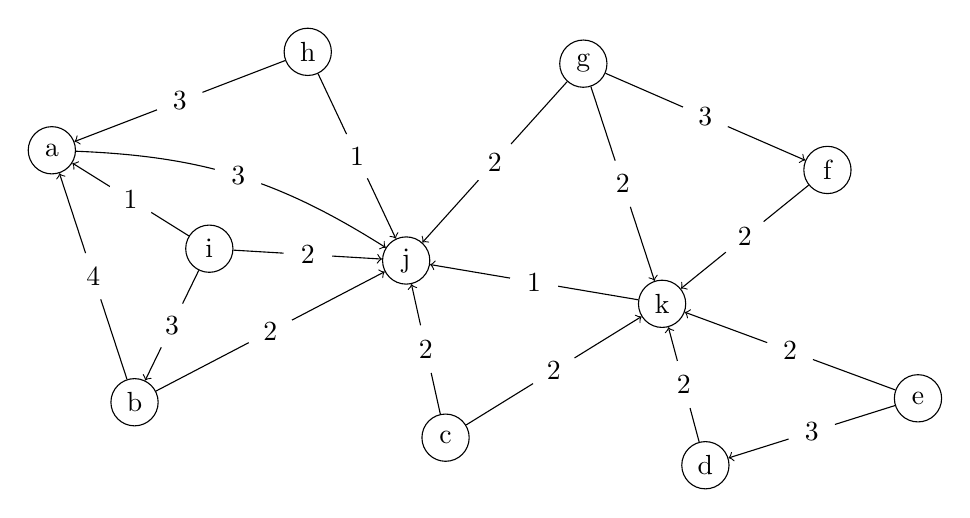
\begin{tikzpicture}
    % Nodes
    \node[circle, draw, minimum size=0.6cm, inner sep=0pt] at (0.5* 0.0, 0.5* 8.5) (a) {a};
    \node[circle, draw, minimum size=0.6cm, inner sep=0pt] at (0.5* 2.1, 0.5* 2.1) (b) {b};
    \node[circle, draw, minimum size=0.6cm, inner sep=0pt] at (0.5* 10.0, 0.5* 1.2) (c) {c};
    \node[circle, draw, minimum size=0.6cm, inner sep=0pt] at (0.5* 16.6, 0.5* 0.5) (d) {d};
    \node[circle, draw, minimum size=0.6cm, inner sep=0pt] at (0.5* 22.0, 0.5* 2.2) (e) {e};
    \node[circle, draw, minimum size=0.6cm, inner sep=0pt] at (0.5* 19.7, 0.5* 8.0) (f) {f};
    \node[circle, draw, minimum size=0.6cm, inner sep=0pt] at (0.5* 13.5, 0.5* 10.7) (g) {g};
    \node[circle, draw, minimum size=0.6cm, inner sep=0pt] at (0.5* 6.5, 0.5* 11.0) (h) {h};
    \node[circle, draw, minimum size=0.6cm, inner sep=0pt] at (0.5* 4.0, 0.5* 6.0) (i) {i};
    \node[circle, draw, minimum size=0.6cm, inner sep=0pt] at (0.5* 9.0, 0.5* 5.7) (j) {j};
    \node[circle, draw, minimum size=0.6cm, inner sep=0pt] at (0.5* 15.5, 0.5* 4.6) (k) {k};

    \draw[->] (a) edge[bend left=15] node[circle, fill=white] {3} (j);

    \draw[->] (b) edge node[circle, fill=white] {4} (a);
    \draw[->] (b) edge node[circle, fill=white] {2} (j);

    \draw[->] (c) edge node[circle, fill=white] {2} (j);
    \draw[->] (c) edge node[circle, fill=white] {2} (k);

    \draw[->] (d) edge node[circle, fill=white] {2} (k);

    \draw[->] (e) edge node[circle, fill=white] {3} (d);
    \draw[->] (e) edge node[circle, fill=white] {2} (k);

    \draw[->] (f) edge node[circle, fill=white] {2} (k);

    \draw[->] (g) edge node[circle, fill=white] {3} (f);
    \draw[->] (g) edge node[circle, fill=white] {2} (j);
    \draw[->] (g) edge node[circle, fill=white] {2} (k);

    \draw[->] (h) edge node[circle, fill=white] {3} (a);
    \draw[->] (h) edge node[circle, fill=white] {1} (j);

    \draw[->] (i) edge node[circle, fill=white] {1} (a);
    \draw[->] (i) edge node[circle, fill=white] {3} (b);
    \draw[->] (i) edge node[circle, fill=white] {2} (j);

    \draw[->] (k) edge node[circle, fill=white] {1} (j);
  \end{tikzpicture}
  \caption{Upward-Graph des Beispielgraphs}
  \label{ch::fig::upward_graph}
\end{figure}

Die Definition des Downward-Graphens erfolgt nun analog zu der des Upward-Graphens:

\begin{definition}[Downward-Graph]
  Sei $G = (V, E)$ und ${vtl}$ eine \emph{vertex-to-level} Funktion dazu. Dann ist ein Upward-Graph des transponierten Graphens $G^T$ ein \emph{Downward-Graph} zu $G$.
\end{definition}

Wenn ein Graph ungerichtet ist, dann ist er äquivalent zu seinem transponierten Graphen und dann ist auch der Upward- und Downward-Graph äquivalent.
Daher entspricht \autoref{ch::fig::upward_graph} gleichzeitig auch dem Downward-Graph des Beispielgraphens.
Es ist zu zeigen, dass Anfragen auf einem auf diese Art definiertem Contracted-Graph $C = (G_u, G_d)$ ebenfalls Korrekt sind.

\begin{beweis}[Korrektheit Contracted-Graph Anfrage]
  Da im Upward- und Downward-Graphen nur Kanten existieren, deren Gewicht mindestens dem kürzesten Pfad Abstand der verbundenen Knoten entspricht, kann in $C$ kein Pfad gefunden werden, der nicht auch in $G$ existiert.

  Sei ${sp}_G(s, t)$ der kürzeste $s$-$t$-Pfad auf $G$ der, unter allen kürzesten $s$-$t$-Pfaden, den Knoten $m$ mit dem höchsten Level enthält.
  Erstelle aus diesem Pfad $(s, \dotsc, t)$ zwei Pfade: $(s, \dotsc, m)$ und $(t, \dotsc, m)$.
  Betrachte den Teilpfad $(s, \dotsc, m)$ der Hop-Länge $n_s$.
  Ist $n_s = 1$, so ist nichts weiter zu zeigen.

  Finde nun den ersten Knoten $s'$ nach $s$, für den gilt, dass sein Level größer als das von $s$ ist und zwischen denen auf allen Pfaden nur Knoten kleiner Level liegen.
  Für diesen gibt es nach der Definition des Upward-Graphen eine Kante mit optimalem Gewicht in ihm.
  Wiederhole dies für den Teilpfad $(s', \dotsc, m)$, bis $s' = m$.
  Durch diese Kanten lässt sich $m$ von $s$ aus in $C$ mit optimaler Distanz finden.

  Analog wird für den Teilpfad $(t, \dotsc, m)$ im Downward-Graphen argumentiert.
  \qed
\end{beweis}

Dass nur Kanten $(t, h)$ erstellt werden müssen, wenn $h$ das größte und $t$ das zweitgrößte Level auf allen $t$-$h$-Pfaden hat, ist in \autoref{fig:people:notwendige_kanten} veranschaulicht.
Es muss keine $(u, w)$ Kante erstellt werden, da $w$ über $v$ erreicht werden kann.

\begin{figure}[h!]
  \centering
  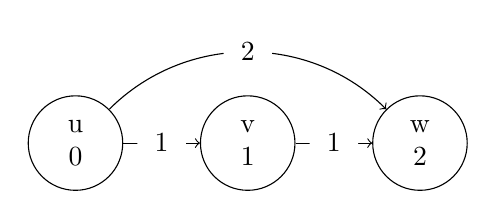
\begin{tikzpicture}[scale=1.75]
    \node[circle, draw, minimum size=1.2cm, inner sep=0pt , align=center] at (0*1.25, 0) (u) {u\\0};
    \node[circle, draw, minimum size=1.2cm, inner sep=0pt , align=center] at (1*1.25, 0) (v) {v\\1};
    \node[circle, draw, minimum size=1.2cm, inner sep=0pt , align=center] at (2*1.25, 0) (w) {w\\2};

    \draw[->] (u) edge[bend left=45] node[circle, fill=white] {2} (w);
    \draw[->] (u) edge node[circle, fill=white] {1} (v);
    \draw[->] (v) edge node[circle, fill=white] {1} (w);
  \end{tikzpicture}
  \caption{Beispiel notwendiger Kanten im Upward-Graph}
  \label{fig:people:notwendige_kanten}
\end{figure}

\subsection{Kontraktion erfüllt diese Definition}

Bei der Knoten-Kontraktion des Knoten $v$ wird für den Pfad $(u, v, w)$ eine Abkürzung eingefügt, wenn dies der einzige kürzeste $u$-$w$-Pfad ist.
Ist dies der Fall, dann wurden die Knoten aller andern kürzesten Pfade zuvor bereits kontrahiert und haben daher ein niedrigeres Level als $u$ und $w$.
Daher bilden diese Abkürzungen mitsamt den Kanten des ursprünglichen Graphen die Kantenmenge des Upward- und Downward-Graphen, wobei die Zuordnung durch die Reihenfolge der Kontraktion von $u$ und $w$ definiert ist.

Wenn die Kontraktionsbedingung abgeschwächt wird, werden nicht notwendige und nicht optimale Kanten eingefügt, dies lässt die Definition aber zu.
Daher entspricht ein durch Graphen-Kontraktion erzeugter Graph der neuen Definition.

\subsection{Algorithmus}

Das Berechnen aller kürzesten Pfade zwischen zwei Knoten ist aufwändig, daher wird zum Berechnen eines so definierten Contracted-Graphens ein ähnlicher Trick angewendet, wie er bei der Knoten-Kontraktion angewandt wird:
Wir fügen Kanten ein, sobald wir \emph{einen} optimalen $t$-$h$-Pfad gefunden haben, auf dem $h$ das größte und $t$ das zweitgrößte Level hat.
Dies ist hinreichend, fügt im Zweifel jedoch mehr Kanten als notwendig ein.

Um einen Upward-Graphen zu berechnen, wird für jeden Knoten $t \in V$ eine angepasste Dijkstra-Suche ausgeführt, bei der für jeden Knoten jeweils notiert wird, was das größte Level auf dem Pfad zur Wurzel ist.
Diese Information kann mit der \emph{max-on-path} Funktion ${mop}$ abegrufen werden.
Ein Knoten $h \in V$, $h \neq t$ ist der Kopf eine Upward-Graph Kante, für die gilt, dass ${mop}(h) = {vtl}(h)$ und ${mop}({pre}(h)) = {vtl}(t)$.
Das Gewicht der Kante kann der Dijkstra Suche entnommen werden.
Die Suche kann abgebrochen werden, wenn nur noch Knoten für alle nicht-expandierten Knoten $h$ gilt, dass ${mop}({pre}(h)) > {vtl}(h)$ ist.
\autoref{ch:fig:ch_brute_force_suchbaum} zeigt dies für den Knoten $a$ im Beispielgraphen.
Die linke Zahl steht dabei für das Level des jeweiligen Knotens, die rechte Zahl für das größte Level auf dem Pfad zur Wurzel.

\begin{figure}[h!]
  \centering
  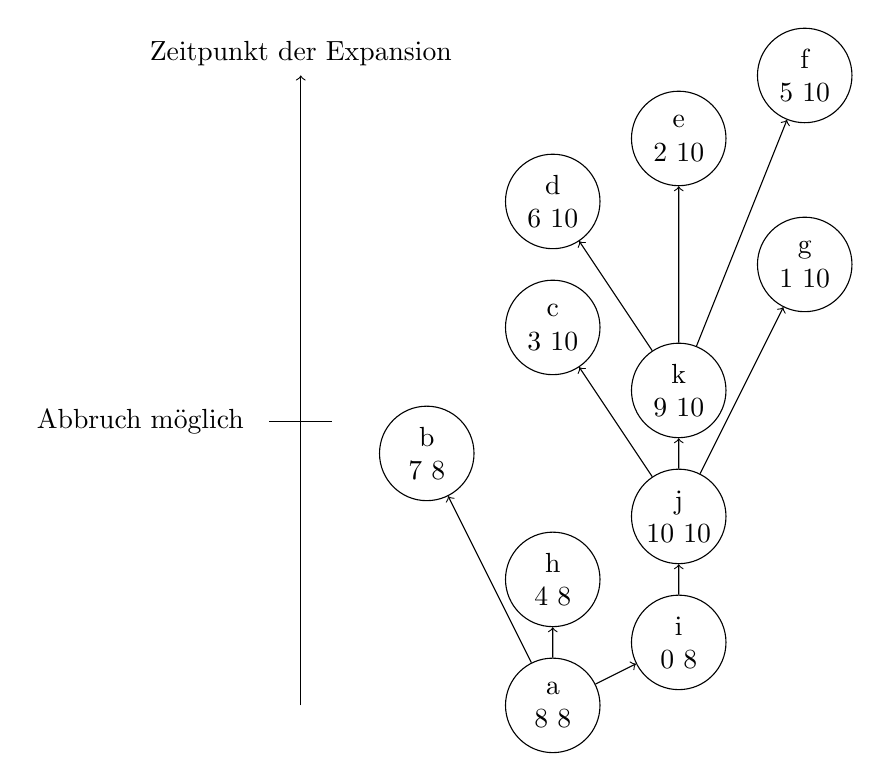
\begin{tikzpicture}[scale=0.8]
    % Nodes
    % a & b & c & d & e & f & g & h & i & j & k &
    % 8 & 7 & 3 & 6 & 2 & 5 & 1 & 4 & 0 & 10 & 9 &

    \node[circle, draw, minimum size=1.2cm, inner sep=0pt , align=center] at (2* 1, 0) (a) {a\\8 8};
    \node[circle, draw, minimum size=1.2cm, inner sep=0pt , align=center] at (2* 0, 4) (b) {b\\7 8};
    \node[circle, draw, minimum size=1.2cm, inner sep=0pt , align=center] at (2* 1, 6) (c) {c\\3 10};
    \node[circle, draw, minimum size=1.2cm, inner sep=0pt , align=center] at (2* 1, 8) (d) {d\\6 10};
    \node[circle, draw, minimum size=1.2cm, inner sep=0pt , align=center] at (2* 2, 9) (e) {e\\2 10};
    \node[circle, draw, minimum size=1.2cm, inner sep=0pt , align=center] at (2* 3, 10) (f) {f\\5 10};
    \node[circle, draw, minimum size=1.2cm, inner sep=0pt , align=center] at (2* 3, 7) (g) {g\\1 10};
    \node[circle, draw, minimum size=1.2cm, inner sep=0pt , align=center] at (2* 1, 2) (h) {h\\4 8};
    \node[circle, draw, minimum size=1.2cm, inner sep=0pt , align=center] at (2* 2, 1) (i) {i\\0 8};
    \node[circle, draw, minimum size=1.2cm, inner sep=0pt , align=center] at (2* 2, 3) (j) {j\\10 10};
    \node[circle, draw, minimum size=1.2cm, inner sep=0pt , align=center] at (2* 2, 5) (k) {k\\9 10};

    \draw[->] (a) edge (b);
    \draw[->] (a) edge (h);
    \draw[->] (a) edge (i);
    \draw[->] (j) edge (c);
    \draw[->] (i) edge (j);
    \draw[->] (k) edge (d);
    \draw[->] (j) edge (k);
    \draw[->] (k) edge (e);
    \draw[->] (k) edge (f);
    \draw[->] (j) edge (g);

    \draw[->] (-2, 0) -- (-2, 10) node[above] {Zeitpunkt der Expansion};

    \draw (-2.5, 4.5) -- (-1.5, 4.5) node[left=1cm] {Abbruch möglich};

  \end{tikzpicture}
  \caption{Contracted-Graph PEOPLE Suchbaum}
  \label{ch:fig:ch_brute_force_suchbaum}
\end{figure}

Die Information des größten Levels auf dem Pfad zur Wurzel kann dabei beim Update eines Knotens übertragen werden, indem das Maximum des bisherigen größten Levels und das Level des upgedateten Knotens gebildet wird.
Die Abbruchbedingung kann durch Betrachtung einer Menge an \emph{lebendigen Knoten} verfolgt werden, sobald diese keine Knoten mehr enthält, kann die Suche abgebrochen werden.
Zu Beginn ist nur der Startknoten lebendig, die Lebendigkeit wird jeweils an die Kinder vererbt.
Ein Knoten stirbt, nachdem er expandiert wurde oder wenn er den Kopf einer Kante bildet.
Gibt es keine lebendigen Knoten mehr, so kann die Suche abgebrochen werden.
In dem Beispiel in \autoref{ch:fig:ch_brute_force_suchbaum} wäre dies etwa nach der Expansion von $b$ der Fall.
Bei einer \emph{guten} vertex-to-level-Funktion ist die Überlegung, dass die Suche früh abgebrochen werden kann.

Die Berechnung ist \emph{embarrassingly parallel}, jeder Knoten kann unabhängig von den anderen berechnet werden.
Der textuell beschriebene Algorithmus wird dann wie folgt formal definiert:

\begin{algorithm}[p]
  \caption{Contracted-Graph PEOPLE Algorithmus}
  \begin{algorithmic}[1]
    \Require Graph $G = (V, E)$, vertex-to-level Funktion ${vtl}$, Knoten $s \in V$
    \Ensure $E_s$
    \State // Initialisiere Distanz- und Vorgänger-Funktion
    \ForAll{$v \in V$}
    \State ${dist}(v) \leftarrow \infty$
    \State ${pre}(v) \leftarrow {none}$
    \EndFor

    \State
    \State // Initialisiere Suche
    \State ${dist}(s) \leftarrow 0$
    \State $Q\leftarrow \{ s \}$
    \State ${pre}(s) \leftarrow s$

    \State
    \State // Initialisiere max-on-path
    \State ${mop}(s) \leftarrow {vtl}(s)$
    \State $E_s \leftarrow \{ \}$
    \State ${alive} \leftarrow \{ s \}$

    \State
    \While{$Q \neq \emptyset \land {alive} \neq \emptyset$}
    \State $u \leftarrow{extract\_min}(Q)$\label{graphs:dijkstra:pop}

    \State
    \State // Beende frühzeitig wenn Zielknoten gefunden wurde
    \If {$u \neq s \land {mop}(u) = {vtl}(u)$}
    \State $E_s \leftarrow E_s \cup \{ (s, u, {dist}(u)) \}$
    \State ${alive} \leftarrow {alive} \setminus \{ s \}$
    \EndIf

    \State
    \State // Aktualisiere Nachbarn
    \ForAll{$(u, v, w) \in E$}
    \If {${dist}(u) + w < {dist}(v)$}
    \State ${dist}(v) \leftarrow {dist}(u) + w$
    \State ${pre}(u) \leftarrow v$
    \State $Q = Q \cup \{ v \}$
    \State
    \State // setze max\_level\_path
    \State ${mop}(v) \leftarrow \max({mop}(v), {vtl}(v))$
    \If {$u \in {alive}$}
    \State ${alive} \leftarrow {alive} \cup \{ s \}$
    \EndIf
    \EndIf
    \EndFor

    \State ${alive} \leftarrow {alive} \setminus \{ s \}$

    \EndWhile

    \State
    \State \Return $E_s$
  \end{algorithmic}
  \label{alg:people:ch}
\end{algorithm}

\subsection{Änderung von Kantengewichten}

Bei Graphen mit hierarchischer Struktur und einer guten Vertex-to-Level-Funktion ist anzunehmen, dass die Suche nach Algorithmus \ref{alg:people:ch}  in den meisten Fällen früh abbricht.
Dies ist einerseits für die Effizienz der Berechnung von Vorteil, verdeutlicht aber auch, dass für die bestimmung der ausgehenden Kanten des Contracted-Graphen für viele Knoten jeweils nur die lokale Umgebung eines Knotens von Bedeutung ist.
Änderungen der Kantengewichte außerhalb dieser Umgebung haben daher in der Regel keinen Einfluss auf die lokale Struktur des Knotens.

Diese Eigenschaft lässt sich nutzen, um nach einer Änderung der Kantengewichte nicht für jeden Knoten sämtliche ausgehenden Kanten neu berechnen zu müssen.
Zwei mögliche Ansätze bieten sich hierfür an:
Zum einen könnte für jeden Knoten gespeichert werden, von welchen Kanten er beeinflusst wird.
Zum anderen könnte für jede Kante berechnet werden, welche Knoten von ihr beeinflusst werden.

Das Speichern des Bereichs, der einen Knoten beeinflusst, kann in Graphen der euklidischen Ebene beispielsweise durch Bounding Boxen realisiert werden. Ob es eine effiziente Methode gibt, mit der der Einflussbereich einer Kante bestimmt werden kann, wird in dieser Arbeit nicht behandelt.

\subsection{Abkürzung Problem}

Es liegt nahe, als abgekürzten Knoten den Knoten mit dem dritthöchsten Level auszuwählen und sich darauf zu verlassen, dass die Suche von diesem Knoten aus die nächste Abkürzung findet, da dies der Knoten-Kontraktion entspricht.
Dies ist praktisch, da dann jeder Shortcut nur einmal erstellt werden muss, dafür muss jedoch gelten, dass die Vorwärtssuche für $s$-$t$ den gleichen Pfad findet wie die Rückwärtssuche (die Suche auf dem transponierten Graphen) für $t$-$s$.
Wird als Graph eine Datenstruktur verwendet, welche die Nachbarn nicht in einer definierten Ordnung ausgibt (etwa eine HashMap), oder eine nicht stabile Prioritätswarteschlange verwendet, ist dies nicht garantiert.

\autoref{ch:fig:problem_shortcut} zeigt eine Situation, in der dies auftreten kann.
In $C$ wurde der Pfad $(a, e)$ gefunden, dessen Abkürzungen jetzt ersetzt werden sollen.
Hierfür wird im ersten Schritt für die Abkürzung $(a, e)$ der abgekürzte Knoten $d$ gefunden, dadurch ist der Pfad $(a, d, e)$.
Wir verlassen uns darauf, dass die Suche von $d$ aus die Abkürzung $(d, a)$ mit dem Knoten $b$ findet, dies geschieht jedoch nicht, wenn $a$ von $d$ aus über $c$ erreicht wird.

\begin{figure}[h!]
  \centering
  \begin{subfigure}[b]{1\textwidth}
    \centering
    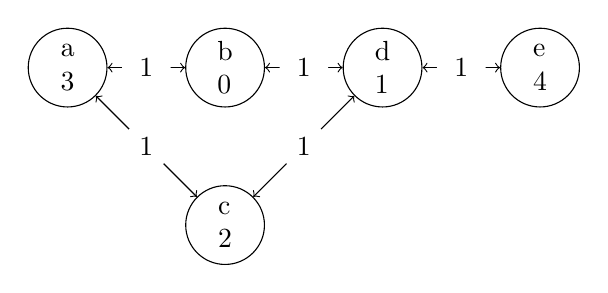
\begin{tikzpicture}
      % Nodes
      \node[circle, draw, minimum size=1cm, inner sep=0pt, align=left] at (2*0, 2*0) (a) {a\\3};
      \node[circle, draw, minimum size=1cm, inner sep=0pt, align=left] at (2*1, 2*0) (b) {b\\0};
      \node[circle, draw, minimum size=1cm, inner sep=0pt, align=left] at (2*1, 2*-1) (c) {c\\2};
      \node[circle, draw, minimum size=1cm, inner sep=0pt, align=left] at (2*2, 2*0) (d) {d\\1};
      \node[circle, draw, minimum size=1cm, inner sep=0pt, align=left] at (2*3, 2*0) (e) {e\\4};

      \draw[<->] (a) edge node[circle, fill=white] {1} (b);
      \draw[<->] (b) edge node[circle, fill=white] {1} (d);
      \draw[<->] (d) edge node[circle, fill=white] {1} (e);

      \draw[<->] (a) edge node[circle, fill=white] {1} (c);
      \draw[<->] (c) edge node[circle, fill=white] {1} (d);
    \end{tikzpicture}
    \caption{Graph}
  \end{subfigure}
  \begin{subfigure}[b]{0.49\textwidth}
    \centering
    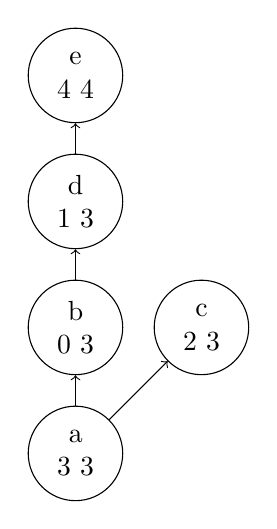
\begin{tikzpicture}[scale=0.8]
      % Nodes
      \node[circle, draw, minimum size=1.2cm, inner sep=0pt, align=center] at (2*0, 2*0) (a) {a\\3 3};
      \node[circle, draw, minimum size=1.2cm, inner sep=0pt, align=center] at (2*0, 2*1) (b) {b\\0 3};
      \node[circle, draw, minimum size=1.2cm, inner sep=0pt, align=center] at (2*1, 2*1) (c) {c\\2 3};
      \node[circle, draw, minimum size=1.2cm, inner sep=0pt, align=center] at (2*0, 2*2) (d) {d\\1 3};
      \node[circle, draw, minimum size=1.2cm, inner sep=0pt, align=center] at (2*0, 2*3) (e) {e\\4 4};

      \draw[->] (a) edge node[] {} (b);
      \draw[->] (b) edge node[] {} (d);
      \draw[->] (d) edge node[] {} (e);
      \draw[->] (a) edge node[] {} (c);
    \end{tikzpicture}
    \caption{Suchbaum von $a$}
  \end{subfigure}
  \hfill
  \begin{subfigure}[b]{0.49\textwidth}
    \centering
    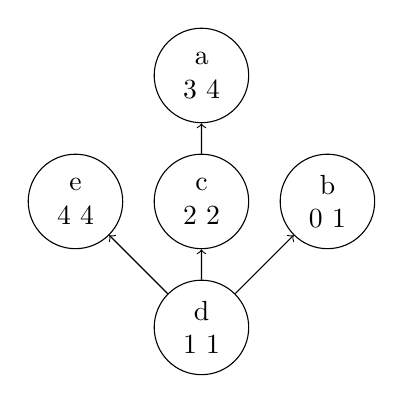
\begin{tikzpicture}[scale=0.8]
      % Nodes
      \node[circle, draw, minimum size=1.2cm, inner sep=0pt, align=center] at (2*1, 2*2) (a) {a\\3 4};
      \node[circle, draw, minimum size=1.2cm, inner sep=0pt, align=center] at (2*2, 2*1) (b) {b\\0 1};
      \node[circle, draw, minimum size=1.2cm, inner sep=0pt, align=center] at (2*1, 2*1) (c) {c\\2 2};
      \node[circle, draw, minimum size=1.2cm, inner sep=0pt, align=center] at (2*1, 2*0) (d) {d\\1 1};
      \node[circle, draw, minimum size=1.2cm, inner sep=0pt, align=center] at (2*0, 2*1) (e) {e\\4 4};

      \draw[->] (d) edge node[] {} (e);
      \draw[->] (d) edge node[] {} (c);
      \draw[->] (d) edge node[] {} (b);
      \draw[->] (c) edge node[] {} (a);
    \end{tikzpicture}
    \caption{Suchbaum von $d$}
  \end{subfigure}
  \caption{Problem beim Shortcut erstellen}
  \label{ch:fig:problem_shortcut}
\end{figure}

Für dieses Problem gibt es zwei Lösungen:
Die nachfolgenden Abkürzungen, welche benötigt werden, um eine Abkürzung vollständig zu entpacken, werden für jede Abkürzung ebenfalls erstellt, dadurch werden viele Abkürzungen mehrfach erstellt, dies muss daher synchronisiert werden.
Alternativ kann die Prioritätswarteschlange modifiziert werden, indem eine Totalordnung der Knoten bestimmt, in welcher Reihenfolge Knoten gleicher Distanz expandiert werden.

\section{PEOPLE}

Analog zur neuen Definition des Contracted-Graph lässt sich auch der Hub-Graph neu definieren.
Die dafür verwendete Definition des Forward-Labels weicht nur leicht von der des Upward-Graphen ab, lediglich die Anforderung, dass der betrachtete Knoten das zweitgrößte Level hat, entfällt.

\begin{definition}[Forward-Label]
  Sei $G = (V, E)$ und ${vtl}$ eine vertex-to-level Funktion dazu.
  Dann ist $L_f (t) \subset V \times \mathbb{R}$ ein Forward-Label für einen Knoten $t$ in $G$ wenn gilt:

  \begin{itemize}
    \item
          $L_f (t)$ enthält nur Einträge $(h, d)$ mit $h \in V$ und $d \in \mathbb{R}$, für die es einen $t$-$h$ Pfad der Länge $d \geq {spd}_G (t, g)$ gibt, so dass auf ihm $h$ das größte Level hat.

    \item
          $L_f (t)$ enthält alle Einträge $(h, {spd}_G (t, h))$ mit $h \in V$, für die gilt, dass auf \emph{allen} $t$-$h$ Pfaden $h$ das größte Level hat.
  \end{itemize}
\end{definition}


Hierbei ist ein Backward-Label ein Forward-Label des transponierten Graphen $G^T$ .
Die Korrektheit dieser Definition folgt direkt daraus, dass der Knoten mit dem höchsten Level auf einem Pfad im Forward- und Backward-Label liegt.

\subsection{Algorithmus}

Solche Labels können wieder durch Merging aus einem Contracted-Graph erstellt werden, jedoch folgt aus dieser Definition auch direkt die Möglichkeit, das Label eines bestimmten Knotens zu berechnen.
Der dafür verwendete Algorithmus ist in Algorithmus \ref{alg:people:people} gelistet, er erzeugt ein gepruntes Label, da er aus Suchbaum auf $G$ das Label erzeugt.

Ein Beispiel einer solche Suche ist in \autoref{ch:fig:hl_brute_force_suchbaum} gezeichnet, dieses verwendet den Beispielgraph, aber nicht die gleiche vertex-to-level-Funktion wie in \autoref{ch::fig::vtl_abbildung}.
Das Label für $a$ enthält $j$, $f$ und $a$ selbst, da ihr Level das jeweils größte auf dem Pfad zur Wurzel ist.

\begin{figure}[h!]
  \centering
  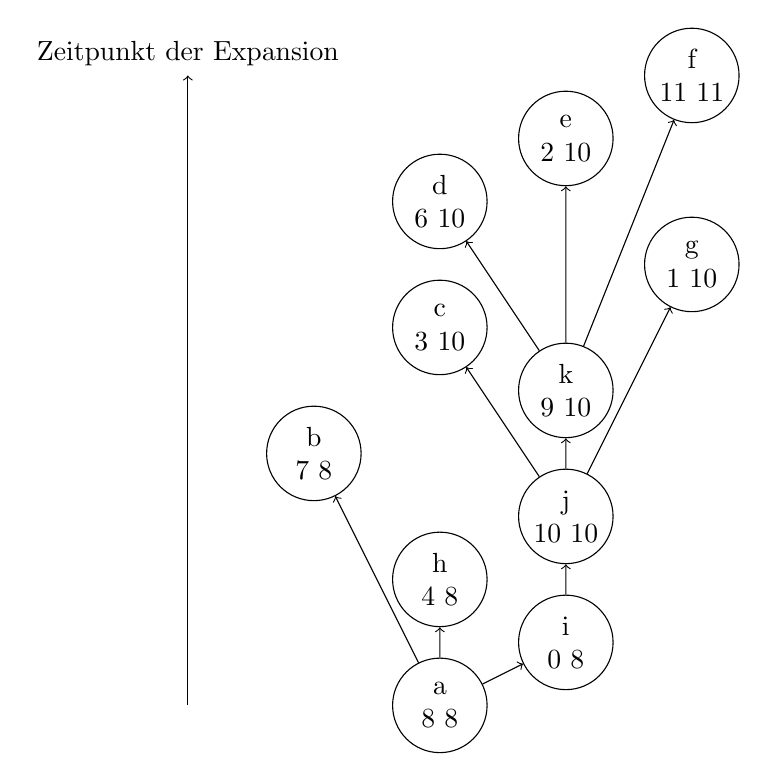
\begin{tikzpicture}[scale=0.8]
    % Nodes
    % a & b & c & d & e & f & g & h & i & j & k &
    % 8 & 7 & 3 & 6 & 2 & 5 & 1 & 4 & 0 & 10 & 9 &

    \node[circle, draw, minimum size=1.2cm, inner sep=0pt , align=center] at (2* 1, 0) (a) {a\\8 8};
    \node[circle, draw, minimum size=1.2cm, inner sep=0pt , align=center] at (2* 0, 4) (b) {b\\7 8};
    \node[circle, draw, minimum size=1.2cm, inner sep=0pt , align=center] at (2* 1, 6) (c) {c\\3 10};
    \node[circle, draw, minimum size=1.2cm, inner sep=0pt , align=center] at (2* 1, 8) (d) {d\\6 10};
    \node[circle, draw, minimum size=1.2cm, inner sep=0pt , align=center] at (2* 2, 9) (e) {e\\2 10};
    \node[circle, draw, minimum size=1.2cm, inner sep=0pt , align=center] at (2* 3, 10) (f) {f\\11 11};
    \node[circle, draw, minimum size=1.2cm, inner sep=0pt , align=center] at (2* 3, 7) (g) {g\\1 10};
    \node[circle, draw, minimum size=1.2cm, inner sep=0pt , align=center] at (2* 1, 2) (h) {h\\4 8};
    \node[circle, draw, minimum size=1.2cm, inner sep=0pt , align=center] at (2* 2, 1) (i) {i\\0 8};
    \node[circle, draw, minimum size=1.2cm, inner sep=0pt , align=center] at (2* 2, 3) (j) {j\\10 10};
    \node[circle, draw, minimum size=1.2cm, inner sep=0pt , align=center] at (2* 2, 5) (k) {k\\9 10};

    \draw[->] (a) edge (b);
    \draw[->] (a) edge (h);
    \draw[->] (a) edge (i);
    \draw[->] (j) edge (c);
    \draw[->] (i) edge (j);
    \draw[->] (k) edge (d);
    \draw[->] (j) edge (k);
    \draw[->] (k) edge (e);
    \draw[->] (k) edge (f);
    \draw[->] (j) edge (g);

    \draw[->] (-2, 0) -- (-2, 10) node[above] {Zeitpunkt der Expansion};

  \end{tikzpicture}
  \caption{Hub-Graph People Suchbaum}
  \label{ch:fig:hl_brute_force_suchbaum}
\end{figure}

\begin{algorithm}[p]
  \caption{PEOPLE}
  \begin{algorithmic}[1]
    \Require Graph $G = (V, E)$, vertex-to-level Funktion ${vtl}$, Knoten $s \in V$
    \Ensure $L_f (s)$
    \State // Initialisiere Distanz- und Vorgänger-Funktion
    \ForAll{$v \in V$}
    \State ${dist}(v) \leftarrow \infty$
    \State ${pre}(v) \leftarrow {none}$
    \EndFor

    \State
    \State // Initialisiere Suche
    \State ${dist}(s) \leftarrow 0$
    \State $Q\leftarrow \{ s \}$
    \State ${pre}(s) \leftarrow s$

    \State
    \State // Initialisiere max-on-path
    \State ${mop}(s) \leftarrow {vtl}(s)$
    \State $L_f (s) \leftarrow \{ \}$

    \State
    \While{$Q \neq \emptyset$}
    \State $u \leftarrow{extract\_min}(Q)$\label{graphs:dijkstra:pop}

    \State
    \State // Beende frühzeitig wenn Zielknoten gefunden wurde
    \If {${mop}(u) = {vtl}(u)$}
    \State $L_f (s) \leftarrow L_f (s) \cup \{ (u, {dist}(u)) \}$
    \EndIf

    \State
    \State // Aktualisiere Nachbarn
    \ForAll{$(u, v, w) \in E$}
    \If {${dist}(u) + w < {dist}(v)$}
    \State ${dist}(v) \leftarrow {dist}(u) + w$
    \State ${pre}(u) \leftarrow v$
    \State $Q = Q \cup \{ v \}$
    \State
    \State // setze max\_level\_path
    \State ${mop}(v) \leftarrow \max({mop}(v), {vtl}(v))$
    \EndIf
    \EndFor

    \EndWhile

    \State
    \State \Return $L_f (s)$
  \end{algorithmic}
  \label{alg:people:people}
\end{algorithm}

\subsection{Anwendungsgebiet}

Die Berechnung der Graphen-Kontraktion in Straßennetzwerken ist in vertretbarer Zeit möglich, jedoch gilt dies nicht für alle Graphenklassen. Insbesondere bei Graphen mit hohem durchschnittlichen Knotengrad stellt die Dijkstra-Suche für jeden Vorgänger einen signifikanten Kostenfaktor dar, sodass die Berechnung der Labels mittels PEOPLE effizienter sein kann.
Da die Labels parallel berechnet werden können, ist es durch den Einsatz geeigneter Hardware möglich, die Berechnungszeit für alle Labels deutlich zu reduzieren.

Der Algorithmus kann auch dazu verwendet werden, die Ergebnisse einer $s$-$t$-Anfrage effizient zwischenzuspeichern.
Falls die Labels von $s$ und $t$ noch nicht vorhanden sind, werden sie im Rahmen der Anfrage generiert.
Nachfolgende Anfragen können dann direkt auf die gespeicherten Labels zugreifen.

PEOPLE kann auch dafür benutzt werden, die durch eine vertex-to-level-Funktion induzierte durschnitliche Label Größe anzugeben, ohne zuerst den Contracted-Graph und anschließend den Hub-Graphen zu berechnen.
Hierfür wird für $n$ Knoten das Label berechnet und über diese die durchschnittliche Größe des Labels angegeben.
Da sich dies leicht parallelisieren lässt, könnte in einem zukünftigen Schritt durch Optimierungsalgorithmen die Label Größe verkleinert werden.